% hc2hp-2.tex

\documentclass[tikz]{standalone}
\usetikzlibrary{positioning, fit}

\begin{document}
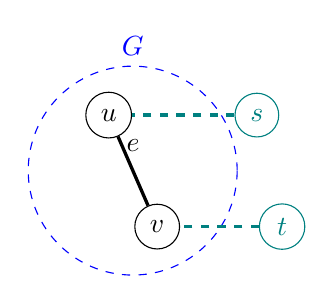
\begin{tikzpicture}[n/.style = {draw, circle, minimum size = 8pt}, 
  every edge/.style = {draw, very thick}]
  \node (u) [n] {$u$};
  \node (v) [n, below right = 1.0cm and 0.2cm of u] {$v$};

  \path (u) edge node [midway, above = 3pt] {$e$} (v);

  \node (g) [draw, dashed, blue, circle, minimum size = 20pt, fit = (u) (v), label = {[blue] above : $G$}] {};

  \node (s) [n, teal, right = 1.3cm of u] {$s$};
  \node (t) [n, teal, right = of v] {$t$};
  \path (s) edge[teal, dashed] (u)
		(t) edge[teal, dashed] (v);
\end{tikzpicture}
\end{document}
